\section{Protein synthesis}

Lastly, we turn our attention to the process of translation. So far in our
estimates there has been little to suggest any apparent limit on the cell's
ability to produce the required number protein species. Even in our example of
\textit{E. coli} grown under different carbohydrate sources
(\FIG{carbon_tport}(B)), cells are able to utilize alternative carbon sources by
inducing the expression of additional membrane transporters and enzymes. For a
doubling time of 5000 seconds, \textit{E. coli} has roughly 3 x 10$^6$ proteins
per cell, which for an average protein of 300 aa, amounts to $\approx$ 10$^9$
peptide bonds that must be formed. This also corresponds to the number of
amino-acyl tRNA that are used, with the pool of tRNA continuously recharged with
new amino acids by tRNA synthetases. At a rate of charging of about 20
amino-acyl tRNA per second (BNID: 105279, \cite{milo2010}), we find that cells
have more than sufficient tRNA synthetases to provide the required amino-acyl
tRNA that are then consumed by ribosomes \FIG{protein_synthesis}(A).

\begin{figure}
    \begin{fullwidth}
    \centering{
        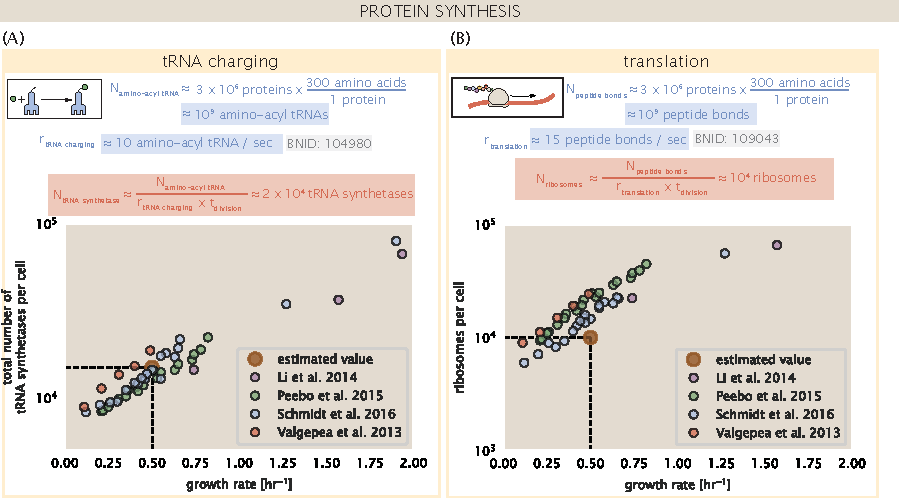
\includegraphics{main_figs/protein_synthesis.pdf}
        \caption{\textbf{Estimation of the required tRNA synthetases and
        ribosomes.} (A) Estimation for the
        number of tRNA synthetases that will supply the required amino acid
        demand. The sum of all tRNA synthetases copy numbers are plotted as a
        function of growth rate ([ArgS], [CysS], [GlnS], [GltX], [IleS], [LeuS],
        [ValS], [AlaS]$_2$, [AsnS]$_2$, [AspS]$_2$, [TyrS]$_2$, [TrpS]$_2$,
        [ThrS]$_2$, [SerS]$_2$, [ProS]$_2$, [PheS]$_2$[PheT]$_2$, [MetG]$_2$,
        [lysS]$_2$, [HisS]$_2$, [GlyS]$_2$[GlyQ]$_2$). (B) Estimation for the
        number of ribosomes required to synthesize all proteins in the cell. The
        average abundance of ribosomes is plotted as a function of growth rate.
        Our estimated values are shown for a growth rate of 0.5 hr$^{-1}$.}
    \label{fig:protein_synthesis}
    }
    \end{fullwidth}
\end{figure}

If we consider a translation elongation rate of $\approx$ 15 peptide bonds per
second (BNID: 114271, \cite{milo2010, dai2016}) cell needs 1.5 x 10$^4$
ribosomes per cell at a growth rate of 0.5 hr$^{-1}$. This is indeed consistent
with the experimental data shown in \FIG{protein_synthesis}(B). From the
perspective of asking whether the process of translation might be rate-limiting,
it is useful to note that the core ribosomal proteins take up as much as []
percent of proteome at the fastest growth rates we have data on. This is in
addition to other ribosomal proteins like the translation elongation factor
EF-Tu that is among the most highly expressed protein. One additional
observation we made earlier in our estimation of rRNA, was that the rRNA operons
need to be nearly packed with transcribing RNA polymerase in order to provide
the required rRNA for each ribosome even at the slower growth rate considered in
our earlier estimate. Experimentally, consecutive deletion of rRNA operons
showed a significant reduction in growth rate in rich media when cells had only
3 or less \citep{levin2017}. Separately, it has been found that gross
overexpression of a protein can dramatically lower growth rate due to the
altered allocation of resources \citep{basan2015}. Optimal resource allocation
and how it relates to cell growth has been an area of intense quantitative study
over the last decade by Hwa and others \citep{scott2010, hui2015}.

We can begin to gain some intuition into how translation, or ribosomes more
specifically, might limit growth by noting that the total number of peptide
bonds generated as the cell doubles, $N_{aa}$, will be given by, $\tau \cdot r_t
\cdot R$. Here, $\tau$ refers to the doubling time of the cell under
steady-state growth, $r_t$ is the maximum translation rate, and $R$ is the
average number of ribosomes in the cell. With the growth rate related to the
cell doubling time by $\lambda = ln(2)/\tau$, we can write the
translation-limited growth rate as,

\begin{equation}
\lambda_{\textrm{translation-limited}} = \frac{ln(2) \cdot r_t \cdot R}{N_{aa}}.
\end{equation}
Alternatively, since $N_{aa}$ is related to the total protein mass through the
molecular weight of each protein, we can also consider the growth rate in terms
of ribosomal mass fraction. An approximation, assuming an average amino acid molecular
weight of 110 Da is shown in \FIG{translation_1}(A).
This allows us to rewrite the growth rate as,

\begin{equation}
\lambda_{\textrm{translation-limited}} \approx \frac{ln(2) \cdot r_t}{L_R}  \Phi_R,
\label{eq:translation_limit_growth_rate}
\end{equation}
where $L_R$ is the total length in amino acids that make up a ribosome, and
$\Phi_R$ is the ribosomal mass fraction. This is plotted as a function of
ribosomal fraction $\Phi_R$ in \FIG{translation_1}(A), where $L_R \approx $8,000 aa,
corresponds to the length in amino
acids for all ribosomal subunits of the 50S and 30S complexes and EF-Tu.

Perhaps the first thing to notice is that there is a maximum growth rate at
about $\lambda \approx 6 hr^{-1}$, or doubling time of about 7 minutes (dashed
line). This growth rate can be viewed as an inherent maximum rate due to
the need for the cell to double the cell's entire ribosomal mass. Interestingly,
this limit is independent of the absolute number of ribosomes, but rather is
simply given by time to translate an entire ribosome, $L_R/ r_t$. As shown in
\FIG{translation_1}(B), we can reconcile this with the observation that in order
to double the average number of ribosomes, each ribosome must produce a second
ribosome. This is a process that cannot be parallelized.

For reasonable values of $\Phi_R$, in the range of about 0.1 - 0.3
\citep{scott2010}, the maximum growth rate is in line with experimentally
reported growth rates around 0.5 - 2 $hr^{-1}$. Here we have implicitly assumed
that translation proceeds randomly, without preference between ribosomal or
non-ribosomal mRNA, which appears reasonable. Importantly, in order for a cell
to scale this limit set by $\Phi_R$ the cell must increase it's ribosomal
abundance, either by synthesizing more ribosomes or reducing the fraction of
non-ribosomal proteins.

\begin{figure}
  \begin{fullwidth}
        \centering{
            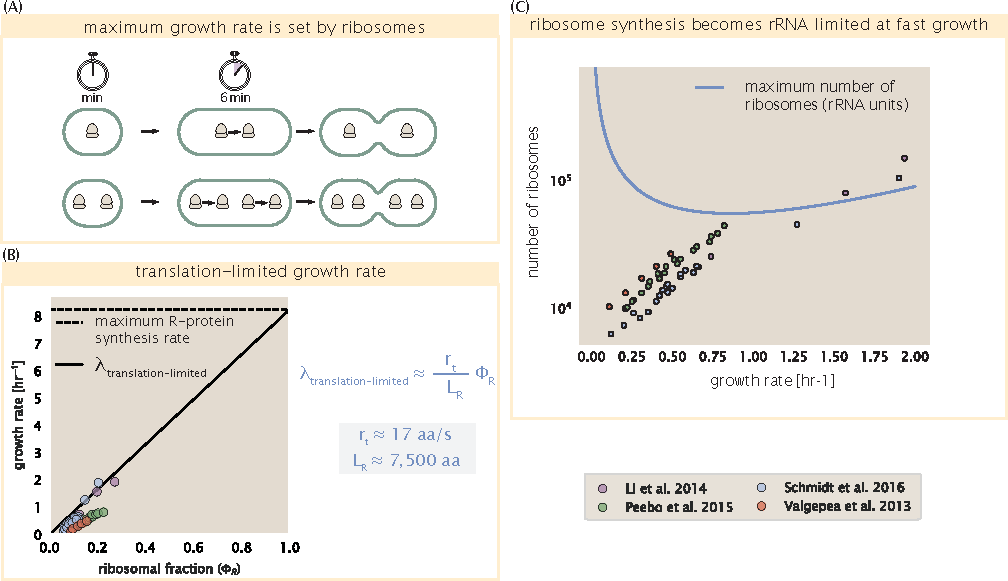
\includegraphics{main_figs/fig7_ribosome_growth_limit_2.pdf}
            \caption{\textbf{Translation-limited growth rate.} (A) Here we
            consider the translation-limited growth as a function of ribosomal
            fraction. By mass balance, the time required to double the entire
            proteome ($N_{aa}$ /$r_t \cdot $) sets the translation-limited
            growth rate, $\lambda_{\textrm{translation-limited}}$. Here $N_{aa}$
            is effectively the number of peptide bonds that must be translated,
            $r_t$ is the translation elongation rate, and $R$ is the number of
            ribosomes. This can also be re-written in terms of the ribosomal
            mass fraction $\Phi_R = m_R$ / $m_{\textrm{protein}}$, where $m_R$
            is the total ribosomal mass and $m_{\textrm{protein}}$ is the mass
            of all proteins in the cell. $L_R$ refers to the summed length of
            the ribosome in amino acids.
            $\lambda_{\textrm{translation-limited}}$ is ploted as a function of
            $\Phi_R$ (solid line). (B) The dashed line in part (A) identifies a
            maximum growth rate that is set by the ribosome. Specifically, this
            growth rate corresponds to the time required to  translation an
            entire ribosome, $L_R/ r_t$ . This is a result that is independent
            of the number of ribosomes in the cell as shown schematically here.
            (C) Schematic showing }
        \label{fig:translation_1}
        }
  \end{fullwidth}
\end{figure}

One last point to note is that across different species of bacteria, while it is
common for bacteria to decrease their ribosomal abundance in poorer nutrient
conditions, this does not decrease to zero \cite{scott2010, liebermeister2014}.
From the perspective of a bacterium dealing with uncertain nutrient conditions,
there is likely a benefit for the cell to maintain some relative fraction of
ribosomes to support rapid growth as nutrient conditions improve. If we consider
a scenario where nutrient conditions become poorer and poorer, there must be a
regime where the cell has more ribosomes than it can utilize. In order for a
cell to maintain steady-state growth, it will need to attenuate its
translational activity since ribosomes would otherwise exhaust their supply of
amino acids and bring cell growth to a halt (\FIG{translation_1}(C)). We will
consider this more specifically for \textit{E. coli} in the next section by considering
recent experimental work.

% In addition,
% given their massive size at about 850 kDa, they may play an as-yet fully
% understood role as a crowding agent in cellular function \cite{delarue2018,
% solerbistue2020}.

\subsection{Multiple replication forks provide a strategy to bias ribosome abundance.}

One feature of \textit{E. coli}, as well as other bacteria like \textit{B.
subtilis}, is their growth by an adder type mechanism whereby cells add a
constant volume with each cell division \citep{taheriaraghi2015}. In conjunction
with this, additional rounds of DNA replication are triggered when cells reach a
critical volume per origin of replication (\FIG{translation_ecoli}(A)). This
leads to the classically-described exponential increase in cell size with growth
rate \cite{schaechter1958, si2017, si2019}. In the context of maximizing growth
rate, it is notable that the majority of ribosomal proteins and rRNA operons are
found closer to the DNA origin, with an increase in rRNA gene dosage needed in
order to meet the demand of an increasingly larger cell at faster growth. This
raises the possibility that the observed global proteome allocation and
specifically, the increased synthesis of ribosomes may be in part a
consequence of increased gene dosage for genes near the DNA origin.

While a bias in gene dosage and transcription is observed for genes near the
origin for rapidly growing \textit{E. coli}  \citep{scholz2019}, we are unaware
of such characterization at the proteomic level. In order to do so with our
data, we calculated a running boxcar average of protein copy number as a
function of the transcriptional start site associated with each protein. While
absolute protein copy numbers vary substantially across the chromosome, we
indeed observe a skew in average protein abundance for genes under the fastest
growth conditions (\FIG{translation_ecoli}(B), showing the result using a 0.5 kb
averaging window). The large positive increases in copy number near the DNA origin
largely reflect an increase in absolute abundance of ribosomal proteins.
This is in contrast to slower growth conditions where the
average copy number is more uniform across the length of the chromosome.

\begin{figure*}
    \begin{fullwidth}
    \centering{
        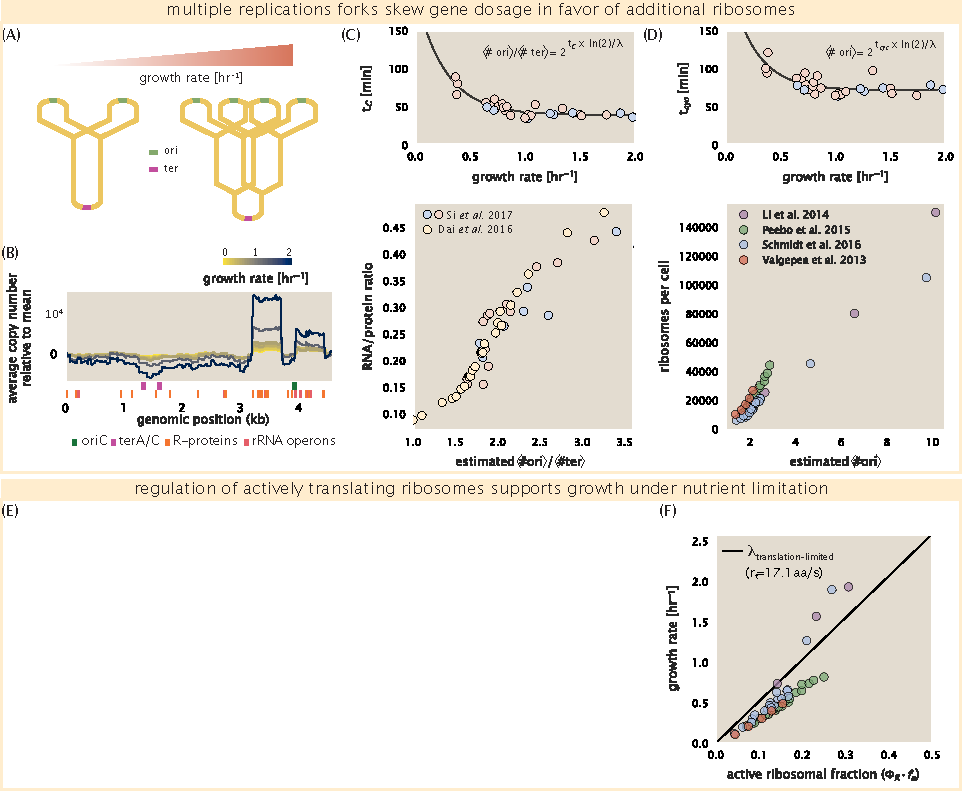
\includegraphics{main_figs/fig8_ribosome_growth_limit_ecoli_temp.pdf}
        \caption{\textbf{Multiple replication forks skew gene dosage and
        ribosomal content.} (A) Schematic shows the expected
        increase in replication forks (or number of ori regions) as \textit{E. coli} cells
        grow faster. (B) The average copy number is calculated at each position along
        the chromosome by running boxcar average with a 0.5 kb averaging window.
        Top plots in (C) and (D) show experimental data from Si \textit{et al.}. (2017)
        Solid lines show fits to the data, which were used to estimate
        $\langle$# ori$\rangle$ / $\langle$# ter$\rangle$ and $\langle$# ori$\rangle$
        [NB: to note fit equations]. Red data points correspond to measurements in strain
        MG1655, while blue points are for strain NCM3722. Bottom plot in (C) compares our estimate of
        $\langle$# ori$\rangle$ / $\langle$# ter$\rangle$  to the experimental
        measurements of ribosomal abundance via RNA/protein ratios. Yellow data points
        correspond to measurements from Dai \textit{et al.} (2016), while the red and blue
        data points come from Si \textit{et al.} (2017).
        The bottom plot in (D) plots the ribosome copy number from the proteomic data against
        our estimate of $\langle$# ori$\rangle$.
        (E) [in progress], (F) Experimenta data from Dai \textit{et al.} are
        used to estimate the fraction of actively translating ribosomes. The
        solid line represents the translation-limited growth rate for ribosomes
        elongating at 17.1 aa/s. }
        \label{fig:translation_ecoli}
    }
    \end{fullwidth}
\end{figure*}

If ribosomal genes (rRNA and ribosomal proteins) are being synthesized according
to their available gene dosage we can make two related hypotheses about how
ribosomal abundance should vary with DNA content. The first is that the
ribosomal protein fraction should increase in proportion  to the average ratio of
DNA origins to DNA termini ($\langle$# ori$\rangle$ / $\langle$# ter$\rangle$
ratio), which is a consequence of the skew in DNA dosage as cells grow faster
that we considered in \FIG{translation_ecoli}(B). The second is that the
absolute number of ribosomes should increase in proportion to the number of DNA
origins ($\langle$# ori$\rangle$), since this will reflect the total gene dosage
in the cell at a particular growth condition.

In order to test these hypotheses we consider the experimental data from Si
\textit{et al.}. $\langle$# ori$\rangle$ / $\langle$# ter$\rangle$ ratio)
depends on how quickly chromosomes ($\tau_C$, referring to the C period of cell
division) are replicated relative the  cell's doubling time $\tau$ and is given
by 2$^{\tau_C / \tau}$ = 2$^{\tau_C \cdot ln(2)/ \lambda}$.  In
\Fig{translation_ecoli}(C)  we plot $\tau_C$ versus $\tau$ that were measured,
with data points in red corresponding to \textit{E. coli} strain MG1655, and
blue  to strain NCM3722. In their work they also measured the total RNA to
protein ratio  which reflects ribosomal abundance and we show that data along
with other recent  measurements from Dai \textit{et al.}. Indeed there appears
to be a strong correlation between ribosomal abundance and the estimated
$\rangle$# ori$\langle$ / $\rangle$# ter$\rangle$. [NB: should I calculate a
correlation coefficient?]. We can similarly estimate $\langle$# ori$\rangle$,
which depends on how often replication forks are initiated per cell cycle. This
is given by the number of overlapping cell cycles,  2$^{\tau_{cyc} / \tau}$ =
2$^{\tau_{cyc} \cdot ln(2)/ \lambda}$, where $\tau_{cyc}$, where $\tau_{cyc}$
refers to the total time of chromosome replication and cell division. The top
plot in \FIG{translation_ecoli}(D) shows the associated data from Si \textit{et
al.}, which we use to estimate $\rangle$# ori$\langle$  for each growth
condition of the proteomic data. In agreement with our expectations, we find a
strong correlation between the ribosome copy number and estimated $\rangle$#
ori$\langle$.

% [NB: to do - 1) slow growth regime, 2) putting it all together - cells appear to
% grow at or near the translation-limited rate (r_t = 17aa/s) across all growth coniditions.]

% [NB: important to highlight - ppGpp null strain abolishes DNA dosage and volume scaling
% ; it also is associated with high # ori/ # ter ]


% ability to begin replication of multiple copies of its genome
% during a single cell cycle. This is achieved through multiple initiation forks
% and nested DNA replication. [need to refer to work from to Jun lab here!! -
% under adder mechanism, the cell appears to add a certain cell mass in proportion
% to its number of origins]. We find that the ribosome copy number increases in
% proportion to the expected number of origins. The process of nested DNA
% replication will lead to a bias in gene dosage for genes closer to the origin of
% replication \cite[], Importantly, ribosomal protein and rRNA genes are closer to
% the origin of replication \cite{scholz2019} and this provides a natural way for
% \textit{E. coli} to bias the proportion of ribosomes at faster growth without
% the advent of additional gene regulation strategies. Given that ribosomal genes
% in \textit{E. coli} appear to be transcribed at their maximal rate at fast
% growth rates [cite??],  increasing ribosomal copy number through increased gene
% dosage represents a creative  approach for the cell to grow faster without gross
% down-regulation of non-ribosomal genes.

% Next consider growth below the capacity of ribosomes.


% Maybe start with E. coli section by noting details from Jun lab as a given. Si et al 2017: The average cell size increased exponentially with respect to the nutrient-imposed growth rate l ( = ln2/t), in agreement with the nutrient growth law [1] (Figure 1; see the Supplemental Information). The ribosome fraction 4R increased linearly with the growth rate, confirming previous re- ports [8, 9]. tC and tcyc were both constant for a wide range of growth conditions at tC = 38.00 ± 4.50 and tcyc = 75.10 ± 7.20 (Fig- ure 1C; see the Supplemental Information) [21, 22].
%  AND it follows 'adder' model of cell division

%  Noting Fig7A, highlight that for cells to optimize their growth , they will benefit by varying their ribosomal abundance; and that they can do this by varying gene dosage - since otherwise it is not obvious how they might make more ribsoomes.

% ****** Data from that 2020 paper on ppGpp and Si et al, and Zhu et al. all point to an increase in ribosomal content with higher number of origins (t_cyc/ tau)
% ->> Can I show this somehow , maybe an important point.



% Might be worth noting that E. coli doesn't grow if you knockout regulation by ppGpp. FROM Zhu et al. 2019 NAR: On the other hand, low ppGpp levels seem to be adverse for biomass growth as well, as shown by the inability of ppGpp- null strain to grow in minimal medium (21,32,33), suggest- ing the importance of maintain an optimal ppGpp level for cell growth.

% It'll remain to be determined whether perturbations like those in Dai et al.,
% and the more recent paper in NAR is consistent with a varying number of
% origins. But I think it's curious that they see a trend exactly like the trend
% in nutrient-limited growth when they vary ppGpp, and roughly similar (high)
% active fraction of ribosomes. I guess is that this type of regulation works
% on more than just ribosomes, and perhaps it is changing number of origins.
% Another point is that fraction of ribosomes again seems to move toward
% a non-zero limit, which bodes well with number of ribosomes depending on
% number of DNA ori.

% I don't think it's trivial to 'up' regulate ribosomal synthensis. This seems like an importsnt consideration.

% I think it might be worth noting that we can think of this changing gene dosage as also changing the genome makeup of the cell.
